% https://www.usenix.org/conference/atc18/requirements-authors

% No longer than 11 pages for full papers, but not including references

% The first page of the paper should include the paper title and author name(s); reviewing is single blind.

% Deadlines

% Paper titles and abstracts due: Tuesday, January 30, 2018
% Complete paper submissions due: Tuesday, February 6, 2018


\documentclass[letterpaper,twocolumn,10pt]{article}
\usepackage{usenix,epsfig,endnotes}
\usepackage{booktabs}

\usepackage[utf8]{inputenc}
\usepackage[T1]{fontenc}

\usepackage[hyphenbreaks]{breakurl}
\usepackage[hyphens]{url}

\usepackage{float}
\usepackage{color}

\newcommand{\mypara}[1]{\vspace{5pt}\noindent{\bf {#1}}}
\newcommand{\red}[1]{\textcolor{red}{#1}}

\newcommand{\note}[1]{\textcolor{blue}{\bf #1}}

\if0
\usepackage{amsmath}
\usepackage{amssymb}
\usepackage{array,booktabs,arydshln}
\usepackage{graphicx}
\usepackage{colortbl}
\usepackage{adjustbox}
\usepackage{multirow}
\usepackage{listings}
\usepackage{pifont}
\usepackage{subcaption}

\newfloat{lstfloat}{t}{lop}
\floatname{lstfloat}{Listing}

\newcommand{\cmark}{\text{\ding{51}}}

\newcommand{\R}{\mathbb{R}}
\DeclareRobustCommand{\rchi}{{\mathpalette\irchi\relax}}
\newcommand{\irchi}[2]{\raisebox{\depth}{$#1\chi$}}

\definecolor{lightgray}{gray}{0.85}

\lstset{frame=tb,
  columns=flexible,
  basicstyle={\scriptsize\ttfamily},
  numbers=none,
  numberstyle=\tiny\color{gray},
  keywordstyle=\color{blue},
  commentstyle={\small\ttfamily},
  stringstyle=\color{mauve},
}

\lstdefinelanguage{Ini}
{
    basicstyle=\ttfamily\small,
    columns=fullflexible,
    morecomment=[s][\color{Orchid}\bfseries]{[}{]},
    morecomment=[l]{\#},
    morecomment=[l]{;},
    commentstyle=\color{gray}\ttfamily,
    morekeywords={},
    otherkeywords={=,:},
    keywordstyle={\color{green}\bfseries}
}
\fi

\begin{document}

%don't want date printed
\date{}

%make title bold and 14 pt font (Latex default is non-bold, 16 pt)
\title{\Large \bf DClaims: Distributed Verifiable Claims for Fake News Detection}

%for single author (just remove % characters)
\author{
  {\rm João Santos}\\
  INESC-ID\\
  ULisboa / Instituto Superior T\'{e}cnico\\
  jrmsantos15@gmail.com
  \and
  {\rm David Dias}\\
  Protocol Labs\\
  mail@daviddias.me
  \and
  {\rm Nuno Santos}\\
  INESC-ID\\
  ULisboa / Instituto Superior T\'{e}cnico\\
  nuno.santos@inesc-id.pt
}

\maketitle

% Use the following at camera-ready time to suppress page numbers.
% Comment it out when you first submit the paper for review.
\thispagestyle{empty}

%!TEX root = ../main.tex

\subsection*{Abstract}

Write me. \note{NS: save it for last.}

%!TEX root = ../main.tex

\section{Introduction}

Write me. \note{NS: save it for last.}

\subsection{Current Shortcommings}
Write me. \note{NS: save it for last.}


\clearpage
%!TEX root = ../main.tex

\section{A primer on the Fake News problem}

Users today when visiting a news outlet or a social network website are commonly confronted with the question as to whether what they are reading is true or false. In this paper, we seek to assist users in tackling this problem by providing a tool to help them spot fake news.

\subsection{News landscape analysis}

Newspapers, magazines and prestigious news outlets have been a reliable news source for centuries. Readers trusted a selected few and the news outlets had an incentive to continue producing good quality information with the risk of loosing their readers to competition. 

Times changed and today.. \note{TODO: present solid references on how the number of news outlets grew, how more fake news are generated and how people trust less and less what they read}

\subsection{Methods used classify Fake News}

\mypara{Content refereeing.} To try to address this problem, some content providers have decided to employ news filtering algorithms for identifying fake news and blocking then from their users. Facebook, Twitter. Facebook has just advertised a system to classify the news based on trustworthiness~\cite{fbrank}. Facebook will begin testing the effort next week by prioritizing news reports in its news feed from publications that users have rated in Facebook surveys as trustworthy. The most ``broadly trusted'' publications—those trusted and recognized by a large cross-section of Facebook users—would get a boost in the news feed, while those that users rate low on trust would be penalized. However, we incur the risks of censorship. Recently, Twitter has been accused of blocking content from right wing circles, and from religious groups. Similar accusation has been made in 2016 to Google, Facebook, and Twitter~\cite{accusedskew}.

\mypara{Fact checkers.} To avoid this, there have appeared services specifically devoted to the identification of fake news and making them available online on some website. Examples of such services include Politifact~\cite{politifact} and FactChecker~\cite{factchecker} focused on US politics, Snopes~\cite{snopes} dedicated to urban myths, and WikiTribune~\cite{wikitribune} to global news. According to a study by the Reuters Institute~\cite{risefackchecking}, in 2016 there were nearly 113 organizations dedicated to fact checking, 90\% of them created since 2010. A fake news organization has even been formed just for this effect, and campaigns for educating users to help them spot fake news. However, the way these systems are build is decoupled from the websites they see, which makes it harder to spot fake news as they visit their preferred news providers. Furthermore, it is sometimes hard for end-users to assess how trustworthy such sources are, making it difficult for users to determine the provenance of the information and reliability of the fact checker. It is sometimes the case that the sources of information are narrowed to specific domains. Another type of system is the Wikipedia, which has already moderation, but relies on a centralized silo of information, with no way for end-users to be able to validate the original provenance of the information.

\mypara{Automatic detection.} There are also emerging automated systems for classifying. But the problem is how to really assess if the results correspond to the truth? It may end up being something where democracy counts. On the other hand it may be possible to build a system where the source of data is already trustworthy and what the system does is to check it. However this is not going to work for real world news where facts have to be validated against external sources before they can be deemed trustworthy. Some previous studies aimed to detect deceptive text on crowdsourced datasets using various techniques, such as stylometric~\cite{stylometric}, semi-supervised learning~\cite{semisupervised}, and linguistic approaches~\cite{linguistic}. Liar~\cite{liar}.

%Centralized solution for someone who stores everything and validates that information for you. Problem of facebook, twitter being accused of bias.

\subsection{A novel approach: Distributed Verifiable Claims}

\note{TODO: João, colocar imagens em papers não funciona como em blog posts. Tu colocas a imagem e tens de fazer referência no texto. Se fores ver a versão render do paper vais ver que a imagem não paarece aqui.}

\begin{figure}[t]
  \centering
  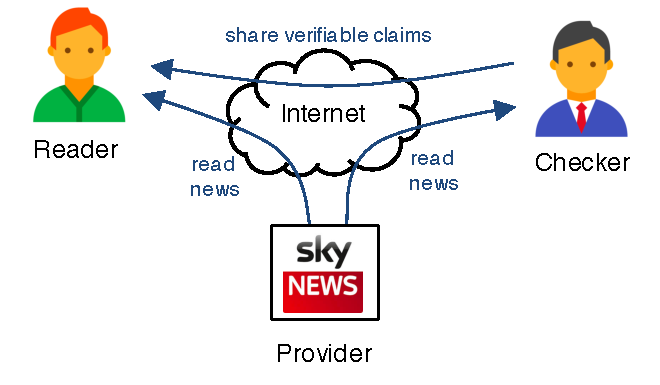
\includegraphics[width=0.9\columnwidth]{figures/model.pdf}
  \vspace{-10pt}
  \caption{Fake news detection based on verifiable claims.}
%  \vspace{-0.3cm}
  \label{fig:model}
\end{figure}

Verifiable Claims are a proposal by W3C. 

\note{TODO:
  - Explicar o que são as Verifiable Claims e fazer ref ao RFC
  - Explicar os shortcommings (json-ld schemas === não funciona offline)
  - Explicar que continua a exigir uma autoridade para guardar as claims
  - Introduzir então as Distributed Verifiable Claims que usam "bleeding edge" e novel approach das Blockchains e P2P para permitir que funcione tudo distribuido
}

\subsection{Requirements}

In order to build a system for fake news detection based on verifiable claims, several challenges need to be overcome:

\mypara{Censorship resistance:} How to prevent someone from blocking access to the content or preventing issuers from submitting their reviews to the system.

\mypara{Security:} How to ensure that the news are not altered, that the content is not modified, and that it is possible for users to be sure that a certain given content has been endorsed by someone they really trust.

\mypara{Resilience:} We need to ensure that our system survives attacks from powerful organizations and is able to preserve the content persistently for a long time span.

\mypara{Source anonymity:} How to provide anonymity protection? Talk about privacy. 

\mypara{Incentives} Talk about incentives that must be aligned. Talk about sustainability.

%!TEX root = ../main.tex

\section{Related Work}

\note{NS: @João please provide your text about the related work.}

\subsection{Overview of the Blockchain Technology}
%\subsection{Trust Decentralisation Through Blockchain}
\label{rel:bitcoin}

\noindent In this section we present the emerging blockchain technology, which is a building block of both Blockcerts and Hypercerts, our proposed system. We start by providing a brief historical context of blockchain (Section~\ref{sec:hist}). Then, we discuss the main features of blockchain as it appeared firstly in the Bitcoin crypto-currency (Section~\ref{sec:tech_bitcoin}), and how it has been improved in alternative crypto-currency systems (Section~\ref{rel:alt-coins}). Lastly, we introduce two relevant systems of the blockchain ecosystem: Ethereum (Section~\ref{rel:ethereum}) and IPFS (Section~\ref{rel:ipfs}), both of which will be used to build our proposed non-siloed certification service.

\subsubsection{Historical Context of Blockchain}
\label{sec:hist}

Blockchain technology was made popular with the creation of Bitcoin \cite{Anonymous:JOJGrvgg}, in 2009. Since the 1980s that there had been proposals for crypto-currency systems and in 2005 for decentralised consensus protocols. The proposed crypto-currency systems were never widely adopted due to the need of a centralised platform, as for the decentralised consensus protocols, they never became a reality as it was unclear how to carry out the implementation. Bitcoin's white paper,\cite{Anonymous:JOJGrvgg}, was published in 2009 by Satoshi Nakamoto (a pseudonym) and it was the first successful implementation of a decentralised crypto-currency system.

Bitcoin was the first truly decentralised crypto-currency, it uses cryptographic properties to solve the double-spending problem \footnote{\url{https://en.bitcoin.it/wiki/Double-spending}} and allows for parties to engage in transactions without having to trust each other. In the backbone of Bitcoin lies a blockchain, which is a distributed ledger that keeps track of every valid transaction that ever took place in the network. Transactions are validated and packed into blocks that are then added to the ledger by nodes (miners) that run a consensus protocol, proof-of-work in the case of Bitcoin. Bitcoin's blockchain has full auditability, meaning that any node can verify the validity of any transaction and correctness, meaning that all the transactions on the longer chain are valid.

The introduction of a blockchain in the Bitcoin design constituted a true technical breakthrough. Although the blockchain concept is mostly associated with Bitcoin, since it played a pivotal role in the large scale adoption of blockchain technology, it has been applied to multiple uses, which range from Internet of Things applications~\cite{Christidis:2016bn}, to new Byzantine Fault Tolerant protocols~\cite{Miller:2016wo}, to alternative crypto-currency systems. With this regard, Bonneau et al.~\cite{Bonneau:2015ema} offer a technical overview on Bitcoin's architecture and protocol, and Barber et al.~\cite{Barber:2012va} identify possible security vulnerabilities and solutions.

%The introduced by Bitcoin was the implementation of a blockchain, a distributed ledger that keeps track of transactions.

%overview of how a blockchain works by using Bitcoin as an example.

%We chose to use Bitcoin as an example because to date, it is the most widespread and tested blockchain and because

\subsubsection{Technical Overview of the Bitcoin's Blockchain}
\label{sec:tech_bitcoin}

Bitcoin proposed an alternative mode of establishing trust between transacting parties. On traditional financial transaction systems, such as banks, two transacting entities have trust on a centralised element, the bank. Let us look at the example of a normal wire-transfer. User A sends money to user B. Both A and B are confident that the bank will withdraw the right amount of money from A's account and place that same amount in B's account. In this traditional trust model the bank is an essential entity in the process as it constitutes the only source of trust between the two transacting parties. Bitcoin's approach is different. Instead of asking the two parties to trust each other, it uses a proof-of-work system whose cryptographic properties assure transactional correctness as long as honest nodes control the majority of the CPU power of the network.

An electronic currency is nothing more than a piece of digital data and one of the features of digital data is their easy replication. For that reason, an issue that an electronic currency has to tackle is the double spending problem. That is, ensuring that a given node is not able to spend the same token (coin) more than once. The way to solve this problem without resorting to a centralised system is to create a ledger of transactions and get all the nodes to agree on the content of that ledger. To that end, a consensus protocol is used, the Bitcoin consensus protocol, also known as the Nakamoto Consensus if based on a proof-of-work.

% \label{rel:bitcoin_proof}
\paragraph{Transactions and proof-of-work:} A Bitcoin transaction consists on nodes exchanging unspent coins and is identified by chain of digital signatures. To complete a transaction the sending node digitally a hash that identifies the past transaction and the public key of the next owner. This ensures that each transaction is linked to the ones preceding it, creating a chain.
The next key challenge is getting all the nodes to agree on the set of past transactions, in order to prevent double-spending.
To that end transactions are packed into blocks, and added to an append-only data structure, the blockchain. Each transaction is linked to the one before it and is signed by the owner of the UTXOs used as input in that transaction.

\paragraph{The mining process:} To add a block to the blockchain, nodes have to mine the block and the way to do that is to solve a mathematical challenge with a pre-defined difficulty level, this is called a proof-of-work~\cite{Gervais:2016dd}. The first node to solve that challenge mines the block, permanently adding it to the Blockchain. Each time a node mines a block, a new Bitcoin (coin) is created and given to that node. This constitutes an incentive for nodes to mine. The algorithm is designed to automatically adjust the challenger's difficulty in order to regulate the currency issuing rate. All the mined blocks are made of transactions that are linked to each other, which means that if a dishonest node was to change a past transaction that change would be eventually be detected by an honest node.

Sometimes a node will mine a block that has already been mined by another node but due to network latency the first is unaware of this. In this situation a fork occurs. Both of these blocks are propagated through the network and eventually a new block will be mined and appended to one of those forks. The network will choose the longest fork as the standing one and the blocks on the branch that is not chosen are discarded. Those blocks are called stale blocks. The probability of the occurrence of a fork of depth $n$ is $O(2^{-n})$ which gives miners a high degree of confidence that the transactions they process will eventually be included in the ledger.

\paragraph{Bitcoin's consensus protocol:} Bonneau et al.~\cite{Bonneau:2015ema} provide an overview of Bitcoin's consensus protocol stability features. It ensures consensus, eventually all correct nodes will agree upon the set of blocks that exist on the blockchain, it has exponential convergence, giving confidence to miners that the blocks they mine will be eventually be added to the blockchain, it has liveness as new blocks will continue to be added, motivating miners by enabling them to collect fees, it has correctness since the longest chain (the active one) will not include stale blocks and it has fairness in the sense that the probability of a miner mine the next block is directly proportional to the amount of computing power that miner has.


\subsubsection{After Bitcoin: Alt-coins and Other Consensus Protocols}
\label{rel:alt-coins}

Following Bitcoin's success, a large and active community has emerged and worked on modifications and extensions to the original protocol to improve some of Bitcoin's shortcomings like performance, introduce new consensus protocols, add new features and even new banking systems~\cite{Danezis:2015ha}. These modifications and extensions, which are usually forks of Bitcoin or abstractions that sit on top of existing blockchains, are called ''alt-coins''~\cite{Bonneau:2015ema}. This section provides an overview of systems that emerged since Bitcoin's inception.

\paragraph{Evening out the distribution of mining power:} One of the criticisms of Bitcoin's proof-of-work mechanism is that is motivates an uneven distribution of mining power. This happens because the time it takes to solve the computational challenge can be decreased by using more CPU cores concurrently. To address this problem, Litecoin\footnote{\url{https://litecoin.org}} introduces a proof-of-work mechanism that is not solved faster by adding CPU cores. Ethereum also tackles this issue (see Section \ref{rel:ethereum}). Other systems propose completely different consensus mechanisms such as proof-of-space~\cite{Dziembowski:2015gs} where nodes are rewarded by storing data, rather than performing computations; this is the case with Permacoin~\cite{Miller:2014kb} and~FileCoin\footnote{\url{https://filecoin.io}} crypto-currency whose goal is to leverage the blockchain to store data. Blockstack~\cite{Ali:2016vq} uses the Bitcoin blockchain to provide a global naming service (like DNS). Peercoin~\cite{King:2012ur} proposes a Proof-of-Stake mechanism where nodes' stake in the network is calculated based on the age of the coins they own and is based on the premise that a node will act in its own best interest, so if has a high stake in the network he will be well behaved and thus contribute to a good operation of the network. DDOS-Coin~\cite{Wustrow:2016tda} proposes a malicious consensus mechanism, proof-of-denial of service, where nodes are rewarded by proving they participated in a DDOS attack. Another consensus mechanism include proof-of-bandwidth~\cite{Ghosh:2014wo}, proof-of-luck~\cite{Milutinovic:2016gs}. Some crypto-currencies proposals have focused on improving Bitcoin's transaction rates and scalability, which is the case of Bitcoin-NG~\cite{Luu:2016cl,Eyal:2016vn}, and others, such as ZCash~\cite{Anonymous:zwRGR7mQ} and HAWK~\cite{Kosba:2016iq}, have focused on transactional privacy~\cite{BenSasson:2015in}.

\paragraph{Enabling contract customisation:} One of the shortcomings of Bitcoin was the lack of contract customisation, as while it did allow for parties to create some rules regarding a given transaction (such as requiring a third party to approve the transaction), doing so required learning a not very intuitive scripting language and the functionality was extremely limited. In particular, it only allowed for a very simple form of smart contracts; smart-contracts are programs that run on the blockchain and allow for the creation of special transaction rules. Ethereum~\cite{Wood:2014ur,Buterin:2013ux} is a crypto-currency blockchain, similar to Bitcoin in many ways, that consists of a smart contract and decentralised application platform. It has a Turing complete programming language which allows for users to create distributed applications while making use of the features of the blockchain.

\subsubsection{Ethereum and Smart-Contracts}
\label{rel:ethereum}

\noindent The alt-coins introduced in the section above aim at solving some of Bitcoin's shortcomings such as scalability and lack of functionality. However, they are highly optimised for one use case and lack flexibility to serve other purposes. Ethereum aims at solving this limitation by offering smart-contracts. A smart-contract is a script that runs in the blockchain. It has Turing completeness, thus effectively offering a state-machine that runs on the blockchain.

Regarding its architecture, Ethereum~\cite{Wood:2014ur,Buterin:2013ux} is built on many of the same principles as Bitcoin. It is a blockchain based system that can also serve as a crypto-currency. It also uses a proof-of-work mechanism as consensus protocol, albeit with a difference, while Bitcoin's consensus protocol challenge lies on CPU power, Ethereum's lies on memory requirement. The goal of this different implementation is to make the network more democratic. One of the consequences of Bitcoin's consensus protocol was the creation of mining farms, i.e., infrastructures provided with Bitcoin mining specialised hardware, which resulted on an uneven distribution of the mining power among active nodes. Memory is something that is extremely optimised on pretty much every electronic device nowadays, much more than CPU power, so this measure should empower lighter miners to the detriment of more powerful ones.

Ethereum provides an API for developers to apply arbitrary logic to smart-contracts. Its transactions can be of one of two types.

\begin{itemize}
\item \textbf{Private}: Are controlled by an Elliptic Curve Cryptography (ECC) private key and allow for currency transaction.
\item \textbf{Smart-contract}: These are transactions controlled by the logic programmed into a smart contract.
\end{itemize}

Both types of transactions can interact with one another (a private transaction can interact with a smart contract and the latter can also engage with a private transaction).
From a programming stand point, one can look at smart-contracts as objects in the Ethereum universe, these objects can interact with each other to fulfil any business rules required by an application.

A smart-contract has to define an upper limit of computing power it will use. This limit of computing power is knows as Gas. The amount of Gas a program has is what defines for how long it can be ran by Ethereum nodes. Gas costs money and miners are rewarded with that Gas. This condition is extremely important to stop programs that halted and malicious programs designed to enter an infinite loop. If a program runs and terminates successfully and does not spend all the Gas, the remainder is returned to the smart-contract, and can be used in future executions. On the other hand if a smart-contract runs out of Gas before ending its execution, all the changes made by the smart-contract are rolled back (to prevent inconsistent states) but the Gas is not returned to the smart-contract, it is given to the miners.

Some of Ethereum's properties can be very useful to build a non-siloed certification service. As described in Section~\ref{revoked}, Blockcerts' current method for verifying if a certificate has been revoked depends on a third party in the sense that it relies on consulting a certificate revocation list which is owned and maintained by the issuer. Ethereum can be utilised to solve this problem. For every certificate, or batch of certificates issued, a smart-contract can be created that keeps track of those certificates' revocation status. The issuer and the receiver would have permissions to change the revocation status of certificates (Section~\ref{proposed:functionalities} details the rationale behind who can revoke certificates) and from there anyone who wanted to verify the revocation status of a given certificate would do so by checking the state of the corresponding smart-contract.

%%%%%%%%%%%%%%%%%%%%%%%%%%%%%%%%%%%%%%%%%%%%%

\subsubsection{The Inter Planetary File System}
\label{rel:ipfs}

Storing data on a blockchain is inefficient and expensive. IPFS is useful for a wide range of applications, one of them being blockchain. IPFS (Interplanetary File System)~\cite{Benet:2014vw} is a peer-to-peer distributed file system. The motivations behind its creation are a better use of bandwidth, the ability to permanently addressing content and moving the web towards a distributed architecture.
As the web grows the amount of bandwidth required to make it work also increases and the HTTP %\footnote{Hypertext Transfer Protocol: https://tools.ietf.org/html/rfc2616}
file transfer model that is widely used today does not optimise bandwidth usage. If 50 people in a classroom all download the same file from Dropbox at the same time, 50 independent requests are made to backbone of the Internet. By addressing that same file with IPFS nodes can download the file from other nodes that have the same file and if there is a node in your network who has the requested file you do not even need an Internet connection. This is a very important feature that can change the way applications work.

Rather than being addressed by their location (IP based link), IPFS files are addressed by their content in the form of a self describing cryptographic hash (a multihash\footnote{\url{https://github.com/multiformats/multihash}}) that is immutable and permanent. This is a desirable feature for Hypercerts as it removes the dependency on an issuer to maintain a link to a file. Thus, to address the storage limitation of blockchains, a user can store large amounts of data on IPFS and reference that data in blockchain transactions, by using the multihash.

IPFS is very efficient in the way it handles data. Each node only needs to store the blocks it is interested in and when a node is searching for a file it queries the network for nodes who have that file. Files are kept track of by using a Merkle DAG~\cite{Merkle:1987jk}, a binary tree where each node is created by hashing its two child nodes, that allows for reliable verification of integrity in large data sets. This is the same data structure behind Git, Bitcoin, and BitTorrent. IPFS is built on top of IPLD, a data format that works as an abstraction layer on top of all the data it represents, which allows for IPFS clients to access data transparently, regardless of the type. This allows for extreme flexibility in the way content is linked, allowing for instance an IPFS client to traverse into an Ethereum smart-contract and check the value of its variables -- in a string based link, just like a file path in a Unix based system -- without the need to run an Ethereum node. Next, we present Blockcerts in more detail.

BlockStack~\cite{blockstack}.

\subsection{Other Refs to Add}
Lottery system using Bitcoin and Ethereum (ieee security symposium) \cite{Miller:2017cf}

Decentralized PKI using blockchain (ieee security symposium) \cite{Anonymous:umr1kkOC}

HAWK: Privacy in smart-contracts using zero knowledge proofs \cite{Kosba:2016iq}




% %!TEX root = ../main.tex

% NOTE: Moved to the end of section 3

%!TEX root = ../main.tex

\section{Architecture}

\begin{figure}[t]
  \centering
  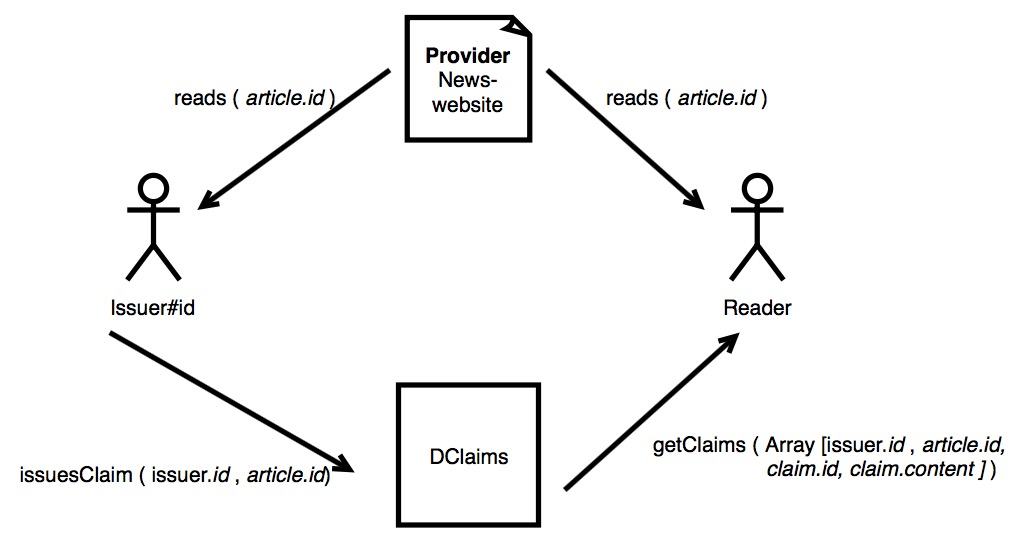
\includegraphics[width=0.8\columnwidth]{figures/arch.jpg}
% \vspace{5pt}
  \caption{DClaims architecture.}
% \vspace{-0.3cm}
  \label{fig:arch}
\end{figure}

Figure~\ref{fig:arch} presents the architecture of our system. 

\note{TODO:
- Need to  explain its core subcomponents: IPFS, Ethereum, and the browser plugin.
- Need to explain why using these components makes sense and discuss alternative approaches.
- Need to introduce two additional parties involved in the system workflow: publishers and curators.}

\subsection{Issuing a Claim flow}

\begin{figure}[t]
  \centering
  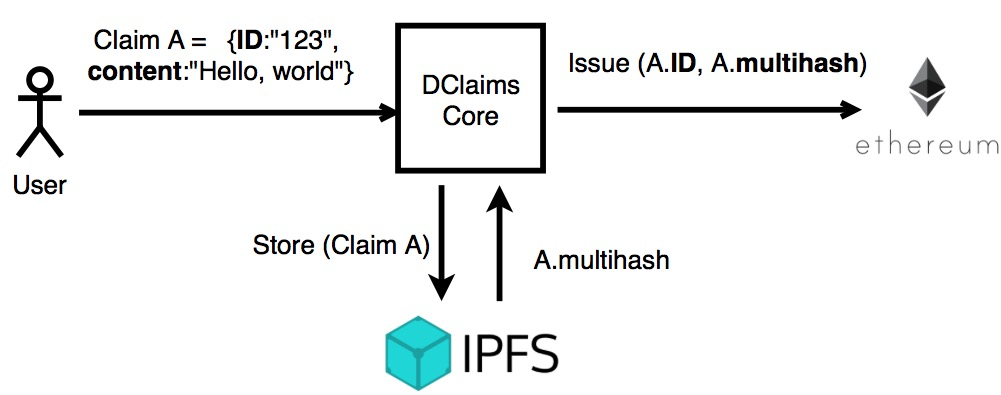
\includegraphics[width=0.8\columnwidth]{figures/arch2.jpg}
%  \vspace{5pt}
  \caption{DClaims issuance workflow.}
%  \vspace{-0.3cm}
  \label{fig:arch2}
\end{figure}

Figure \ref{fig:arch2} shows the issuing process.A user creates a Claim, A, with ID=123 and Content=“Hello, World”, DClaims adds that claim to IPFS, which returns the IPFS link (multihash), DClaims takes that ipfs-link and adds it to the Ethereum smart-contract, indexed by the ID. Meaning that for each ID there can be several claims. (note to self: change id to something better like index)

\subsubsection{Claims Discovery and Propagation}

Claims are stored on IPFS: Distributed file systems, Ensures the links don’t get broken.
An Ethereum smart-contract is used to keep track of the claims, Runs on a blockchain, Allows for the creation of smart-contracts (more about smart-contracts here), Turing complete

\subsection{Threat Model}

\note:{TODO: Here we need to properly characterize the attacker, what he can do, what he cannot do. Talk about what entities we trust.}

\subsection{Issuing and Verifying Claims}

\note:{TODO: Start by explaining the basic process for issuing and verifying claims involving IPFS and Ethereum. Then explain why IPFS and (in particular) Ethereum are important and necessary to make this work. Discuss other potential alternatives.}

\subsection{Costs and Incentives}

\note:{TODO: Here explain that by using Ethereum, costs will be involved. Talk about both the monetary costs of the issuing process and also the performance implications of relying on micro contracts. Then explain the solution based on publishers.}


\subsection{Claim Representation and Aggregation}

\note{TODO: Here explain the basic mechanism for representation of news, graphs between then, attaching more complex types of information, and dealing with a potentially large number of issuers and news. Talk about the curators as a solution for one of these problems.}

\subsection{Supporting Anonymous Sources}

\note{TODO: Talk about anonymous sources and how they can be supported. Talk also about the fact that it is going to be really difficult to revoke claims.}

\subsection{Resistance to censorship}

The application is executed locally, so news websites can not prevent users from running the extension on their website. The most they could do would be to change the name of the HTML classes, but we would quickly catch up.

Someone could still attack IPFS and Ethereum. \note{TODO: explain the thread model}

\subsection{Compatibility}

\note{TODO: Explain how easy it is to make work on any news-website.}

\subsection{Data Model}

Verifiable Claims are a data representation modal, proposed by the W3C Credentials Community Group \footnote{https://web.archive.org/web/20171013165205/https://www.w3.org/TR/verifiable-claims-data-model/} for describing achievements, qualities or other information.

An example would be a university digital diploma, singed by the university’s private key, that I can take to any employer and they can verify it. This diploma should continue to be verifiable even if the university ceases to exist.

Actions supported by Verifiable Claims:

\begin{itemize}
    \item Issue
    \item Share / retrieve
    \item Verify
    \item Revoke
\end{itemize}

What we want to do is to provide a platform that allows end users to have news items automatically reviewed by independent parties of their trust. News are understood as claims which are submitted to a review process. Figure~\ref{fig:model} shows how we envision it working. In our system there are three parties: providers, readers, and issuers. Providers are responsible for serving news content to the users on their browsers. Readers are nothing but the end users which visit providers' websites and browse through the news content. Issuers are responsible for reviewing certain news and issuing a certificate which will be associated to the news.

The idea is that the readers are able to check if some news items is reliable or fake depending on the endorsement produced by some issuer. Readers should be able to designate which issuers they trust so that by the time they visit a given website, each news item is classified according to the review generated by the issuer.

Note that it is not our goal to build a tool that can determine {\em per se} and automatically fake news. Our approach is instead to let readers establish trust relations with someone that they trust to provide them with reliable information. This can be, e.g., some original author, communities of experts, etc. Our system should allow issuers also to attach proofs of what they say is true. Put simply, we want to provide an instrument that can help news readers to mimic trust relations they have in the real world also in the virtual world.

\note{Organize all the stuff below}

\subsection{Publishers}
\label{sec-publishers}

Entities that work as proxies to between issuers and the ethereum network.
Publishers receiver batch claims for a certain news article. When a publisher has receiver X (x being a treshold that can be defined by each publisher)
The single claims are batched into one larger claim, a batch, which is added to IPFS and issued in Ethereum as one transaction, which drops the price. Price of issuing one single claim = price of issuing a batch (which can have any number of single claims).
Publishers can then chose if they want to carry the cost of issuing to the issuers (100 claims from 100 different issuers, the ehthereum transaction price was 1USD, so each issuer would pay 0.01USD) or pay for the issuing themselves by implementing other mechanisms to generate revenue (display ads, have the issuers mine some cryptocurrency for them, mass adoption like review websites).

\paragraph{Misbehaved publishers: } Since publishers act as a proxy between issuers and the Ethereum smart-contract, in theory they could chose not to issue claims that they don’t like, effectively introducing censorship in the system. For that problem we have thought about two solutions, both based on the assumtption that everytime a issuer sends a claim to be issued by a publisher, the publisher replies with a receipt that a) acknowledges having received the claim (eg. returning the claim signed by the publisher) and b) has a prediction of when that claim will be issued (the block interval where that batch might be issued, eg. “your claim will be inserted in the batch with ID=X and should be inserted between blocks 1234567 and 1234590”).

\begin{enumerate}
    \item If the Issuers queries the blocks that he had on the receipt and verifies that the claim has not been inserted there, the Issuer could generate a new claim (issue it directly) where he proves (using the receipt) the publisher misbehaved. That claim could be issued in a “Bad-Publishers” smart-contract, which would warn the community not ti use that specific Publisher.
    \item A more dramatic, but possibly more effective approach would be to have publishers placing money in a smart-contract, as escrow. That smart-contract could receive “complaints” from issuers, which would contain the receipt sent by the publisher to that issuer. The smart-contract could then query the other smart contract (where the claim was supposed to be issued) and check if it had indeed been issued or not. If the smart-contract determined that the issue misbehaved, the value (or part of) the publisher had placed in escrow would be transfered to the complainant issuer. If batches are issued as a merkle tree, the merkle root would be the ipfs link and there is a great optimization that can be done here.
\end{enumerate}

\subsection{Curators}
\label{sec-curators}
Entities that take existing claims and generate new ones, based on the original ones.
Eg. "A Curator finds 100 claims about news article A. He would then issue a new claim saying something like ‘40% of claims classify this article as having a misleading title’ "
This would be useful for the end consumer, who could chose to subscribe to Curators rather than to individual issuers (Looking at a police report vs interviewing all the people involved in an event).

Curators could also create claims about articles that are similar to others.


\subsection{DClaims Web Extension}
\label{sec-web-extension}
The DClaims web extension creates a user interface on any news website that enables users to use the platform.
In its current form the DClaims web extension uses jQuery and Bootstrap for the user interface, Metamask and the Web3 library to communicate with Ethereum and the JS-IPFS-API to communicate with the IPFS daemon.
The DClaims web extension can be adapted to work on any news website with minimal configuration. As we will see in this section, DClaims starts by identifying the news website the user is on and then proceeds to learn if the user is in the website’s homepage or on a full article page.
News articles are identified by their URL and after having gathered the information about the news website and webpage (homepage or full article), DClaims generates IDs for each news article. One of two situations occur, either the user is visiting the homepage of the news website where multiple articles are displayed, or the user is in a full article page. In the first case, homepage, DClaims scrapes the entire webpage and looks for the URLs that each news article references and generates the article ID based on that URL. On the second case, full article page, the ID is generated based on the webpage’s URL (which will be the same that the article on the homepage was referencing). Let us now look into the behaviours in the homepage and full page.

\paragraph{Behaviour News Website’s Homepage}
In the homepage, DClaims enables user to view the claims made about each article displayed. The tasks it has to accomplish on the homepage are creating the visual elements to view claims, and claims count, made about each article. As stated before, the first step is to generate the ID for each article. After that, the HTML Document Object Model (DOM) elements are generated. DOM elements are connected to news articles via their ID, meaning a DOM element’s ID is the same as the ID of the article it serves.
The count of the number of claims is obtained by contacting the smart-contract, via Web3, and querying for that specific article.

\paragraph{Behaviour News Website’s Full Article Pages}
In a full article page, DClaims allows users to generate Claims about that article. As in the case of the homepage, DClaims starts by generating the article ID, followed by the creation of the HTML DOM elements, which in this case are a button to generate a claim and an pop up box with the claim fields to be filled by the user.

\subsection{DClaims Core component}
\label{sec-core}

The DClaims core component handles communication with IPFS and Ethereum and it can run both on a Javascript (browser) or Node.js environment. It can be seen as the backend of the system, even though the concept of backed does not really apply here since we are dealing with a decentralized system.
 It connect to Ethereum using the Web3 object injected by Metamask, in the case of the browser extension, or it can connect directly to a Go-Ethereum (Geth) node, via the RPC.

DClaims core allows for the issuance and retrieval of claims, fetching the claims count for a given article ID and learning the identity of the current user.

\paragraph{Issuing a Claim}
In DClaims news articles are identified by an ID and to issue a claim DClaims receives the Claim object as well as the article id. The Claim object is stored on IPFS which returns the permanent and immutable link. After having the IPFS link, DClaims sends a transaction to the DClaims Ethereum smart-contract which calls the issue function with article ID and IPFS link as parameters. This results in a new entry on the smart-contract’s  articles claims hash list.
DClaims than returns the transaction ID in case the user wants to check the transaction confirmation status.

\paragraph{Getting a claim}
tbd


%!TEX root = ../main.tex

\section{Implementation}

\note{NS: @João explain how the thing is currently implemented. Provide a few snapshots of the system.}


\section{Evaluation}

\note{NS: @João provide a list of the main results we want to add in here.}

\begin{figure}[t]
  \centering 
  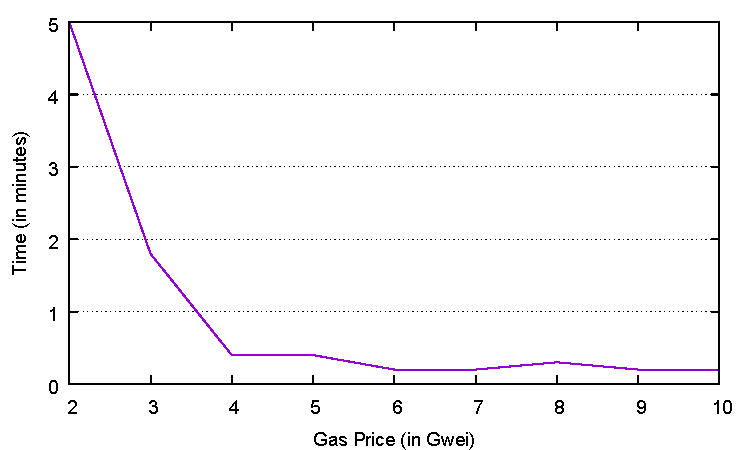
\includegraphics[width=\columnwidth]{final-figures/ethereum-confirmation-time.pdf}
  \vspace{-10pt}
  \caption{Ethereum transaction confirmation time in function of Gas Price.}
%  \vspace{-0.3cm}
  \label{fig:confirmationtime}
\end{figure}

\begin{table}[]
\centering
\begin{tabular}{@{}lll@{}}
\toprule
\textbf{\begin{tabular}[c]{@{}l@{}}Gas price \\ (Gwei)\end{tabular}} & \textbf{\begin{tabular}[c]{@{}l@{}}Contract Creation Cost \\ (in USD)\end{tabular}} & \textbf{\begin{tabular}[c]{@{}l@{}}Claim Issuance Cost\\  (in USD)\end{tabular}} \\ \midrule
\textbf{2}                                                           & 1,72                                                                                & 0,24                                                                             \\
\textbf{4}                                                           & 3,43                                                                                & 0,48                                                                             \\
\textbf{6}                                                           & 5,15                                                                                & 0,72                                                                             \\
\textbf{8}                                                           & 6,86                                                                                & 0,96                                                                             \\
\textbf{10}                                                          & 8,58                                                                                & 1,20                                                                             \\ \bottomrule
\end{tabular}
\caption{DClaims Ethereum Costs}
\label{my-label}
\end{table}



\begin{figure}[t]
  \centering
  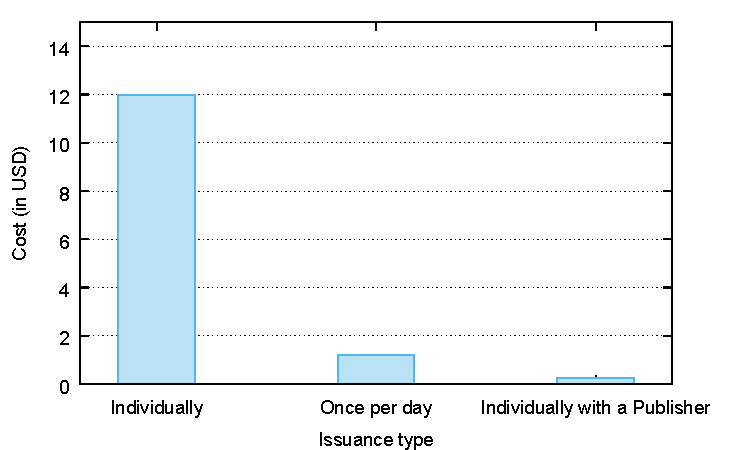
\includegraphics[width=\columnwidth]{final-figures/publisher-issuing-price.pdf}
  \vspace{-10pt}
  \caption{Cost of issuing claims in the different available ways.}
%  \vspace{-0.3cm}
  \label{fig:costpublishers}
\end{figure}

\begin{figure}[t]
  \centering
  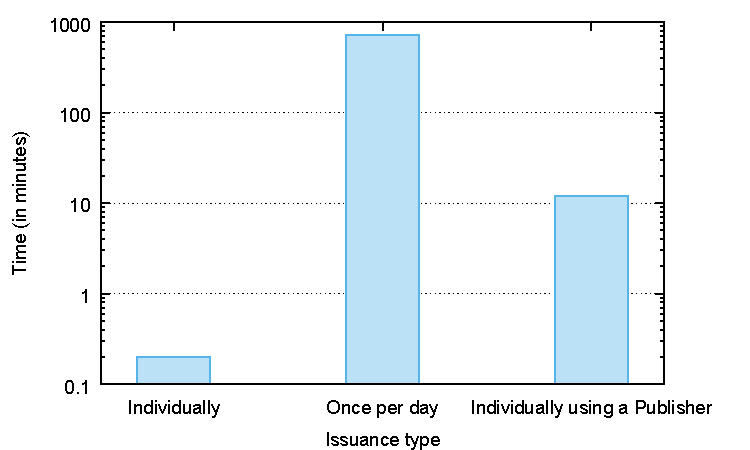
\includegraphics[width=\columnwidth]{final-figures/publisher-issuing-time.pdf}
  \vspace{-10pt}
  \caption{Time for claims to be confirmed on the Ethereum blockchain}
%  \vspace{-0.3cm}
  \label{fig:timepublishers}
\end{figure}

\begin{figure}[t]
  \centering
  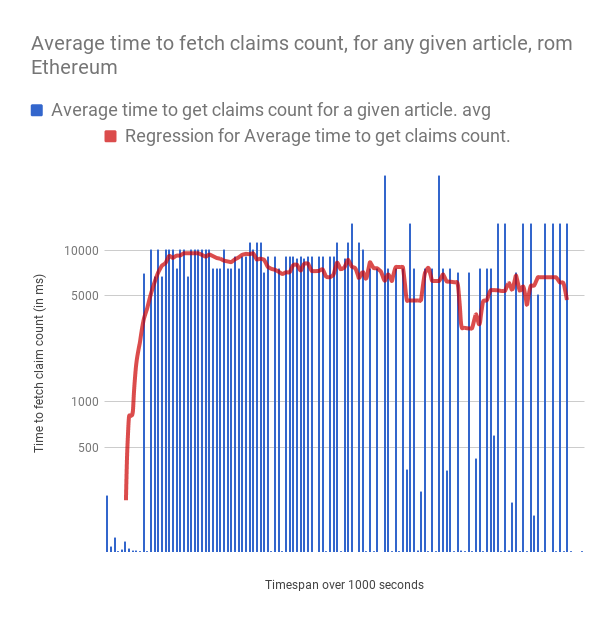
\includegraphics[width=\columnwidth]{mock-figures/ethereumfetch.png}
  \vspace{-10pt}
  \caption{Time to load a webpage as function of the number of articles. \note{NS: @João dont forget to add two curves: one with the other without DClaims.}}
%  \vspace{-0.3cm}
  \label{fig:ethereumfetch}
\end{figure}

\begin{figure}[t]
  \centering
  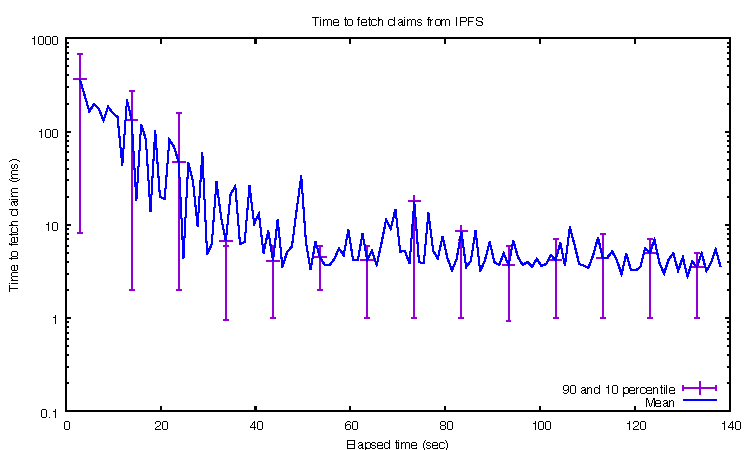
\includegraphics[width=\columnwidth]{mock-figures/ipfsfetch.pdf}
  \vspace{-10pt}
  \caption{Time to fetch individual claims from IPFS}
%  \vspace{-0.3cm}
  \label{fig:ipfsfetch}
\end{figure}

\subsection{Performance of Web Application}


In this section, we evaluate the impact of DClaims in terms of the user experience of the website. \note{NS: @João extend the same experiments for 5 sites, try to pick different sites.}

\begin{figure}[t]
  \centering
  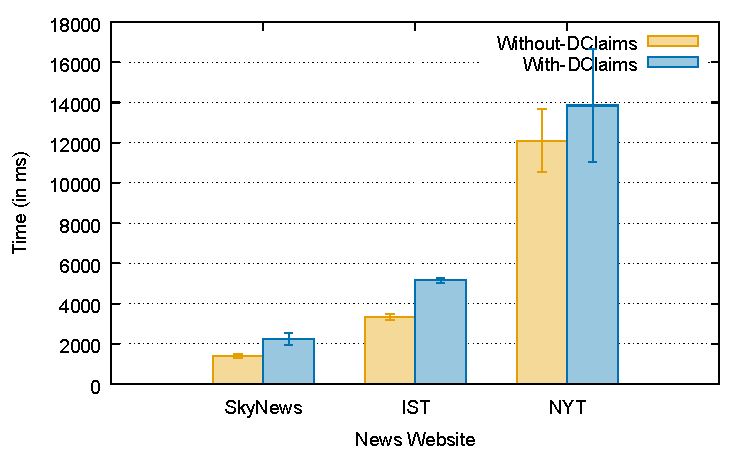
\includegraphics[width=\columnwidth]{final-figures/website-3-comparison.pdf}
  \vspace{-10pt}
  \caption{Loading time comparison of popular news websites with and without DClaims running.}
%  \vspace{-0.3cm}
  \label{fig:evalwebpage}
\end{figure}

\mypara{1. What's the overhead of loading a web page with DClaims?} Figure~\ref{fig:evalwebpage} shows the time it takes to fetch claims from three news websites, Instituto Superior Técnico, SkyNews and New York Times. We can see that the overhead introduced by DClaims is very low.

Figure \ref{fig:evalnarticles} is a benchmark test were we used a striped down version of a website as a basis and created several versions of that website, each with ten more news articles than the previous one. As the figure shows the overhead introduced by DClaims is proportional to the number of articles per page.

By comparing Figures \ref{fig:evalwebpage} and \ref{fig:evalnarticles} one might wonder why in the first, the overhead introduced by DClaims appears to be smaller than in the second. That happens because the website we used for the benchmark has been stripped down of any Javascript code, which slows down the loading time. The same does not happen in regular websites such as SkyNews and the New York Times. 

\note{JS: The conclusion here is that while when compared to super simplified websites, the overhead introduced by DClaims is significant, in the real world it is hardly noticed because regular websites are loaded with JS code that slows down the loading time}

\begin{figure}[t]
  \centering
  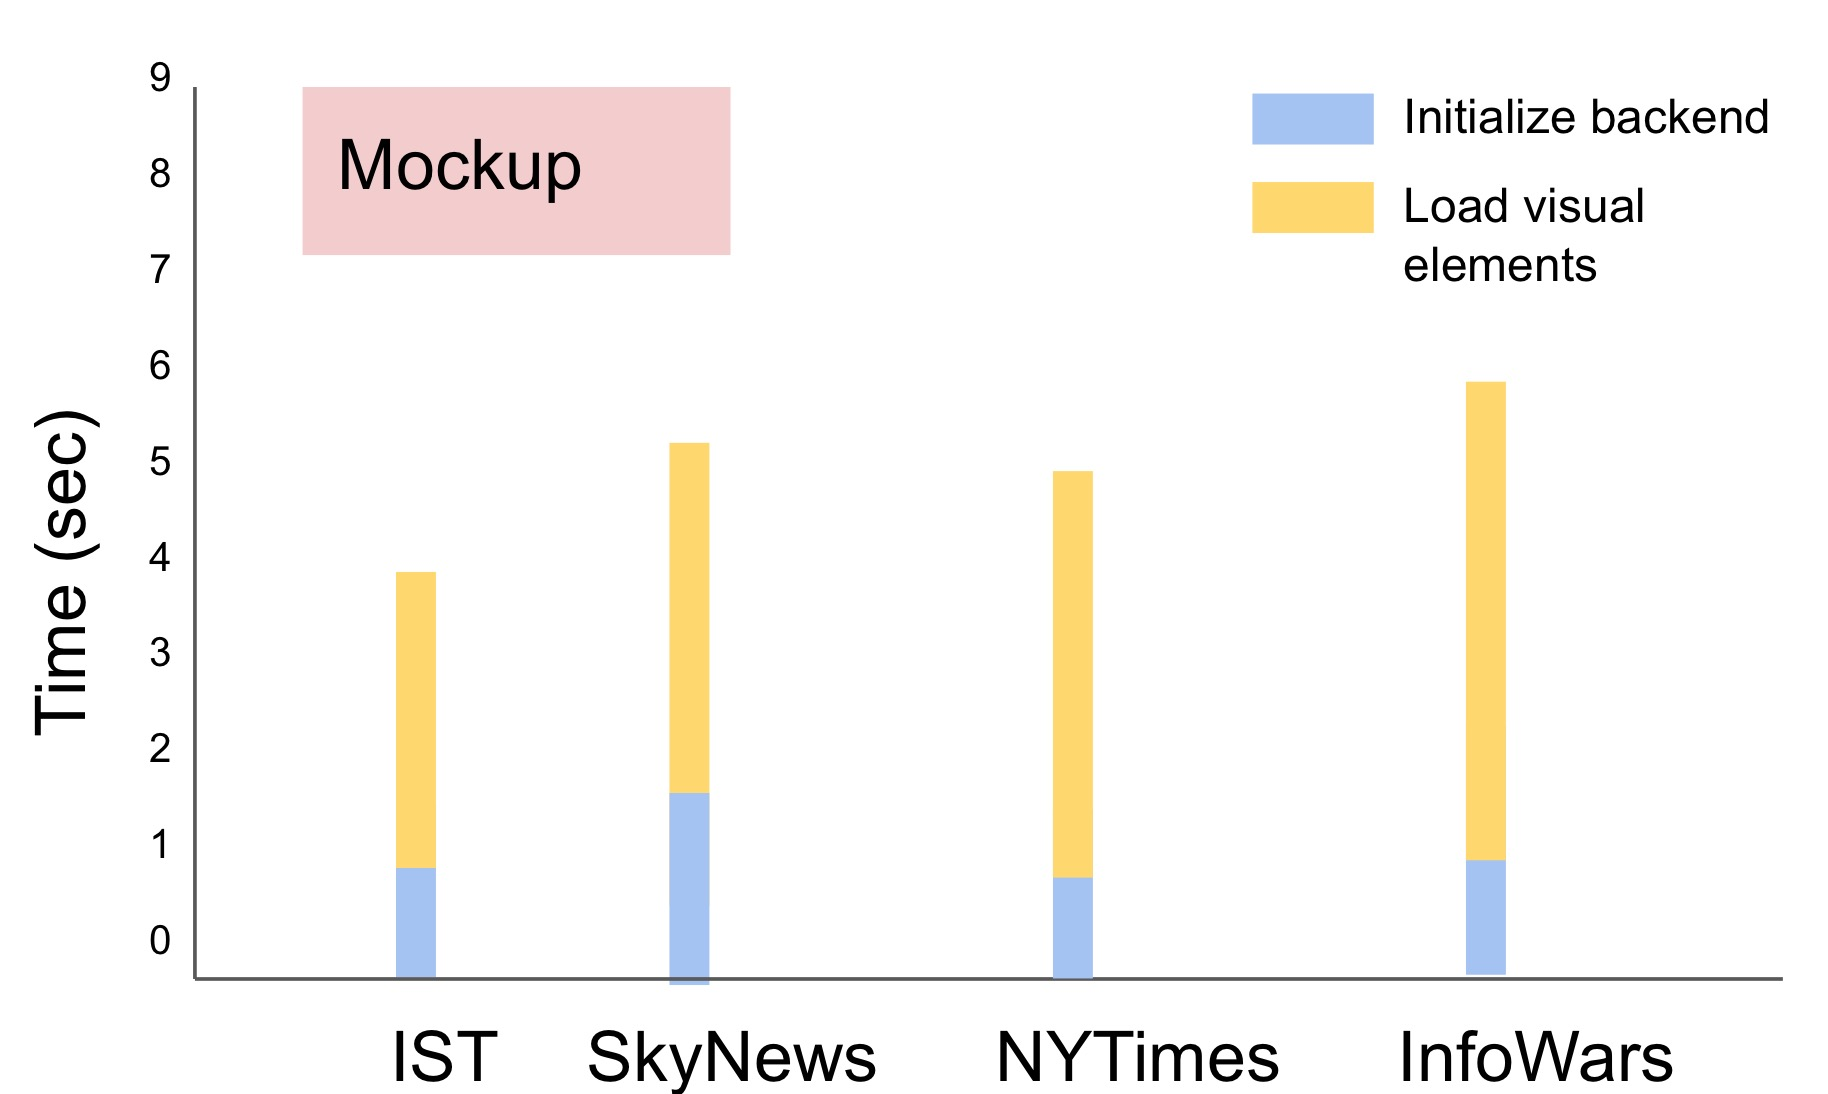
\includegraphics[width=\columnwidth]{mock-figures/timessubcomponents.jpg}
  \vspace{-10pt}
  \caption{Time of drawing the elements and initializing the backend.}
%  \vspace{-0.3cm}
  \label{fig:evalpartial}
\end{figure}

\mypara{2. What is the source of the overheads introduced by DClaims?} Figure~\ref{fig:evalpartial} shows the contributions of two main parts: element drawing and interaction with the backend. \note{NS: @João please change the graph to a compound graph.}
 \note{JS: Didn't have the time to do this one yet}


\begin{figure}[t]
  \centering
  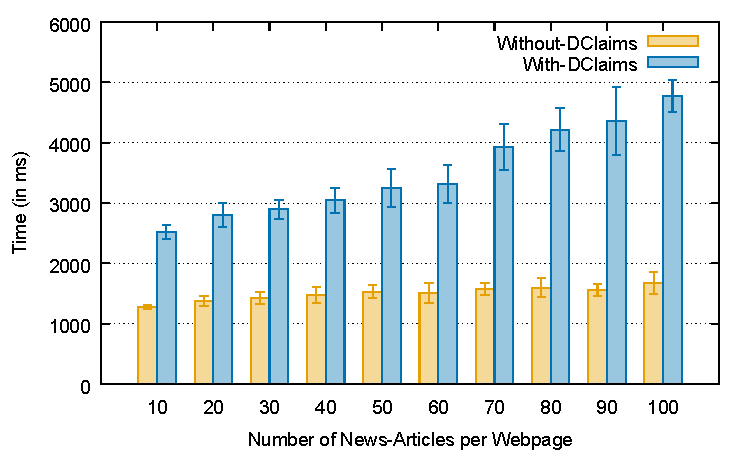
\includegraphics[width=\columnwidth]{final-figures/website-benchmark.pdf}
  \vspace{-10pt}
  \caption{Time to load a webpage as function of the number of articles.}
%  \vspace{-0.3cm}
  \label{fig:evalnarticles}
\end{figure}


\mypara{3. What is the website loading time based on the number of articles in the page?} Figure~\ref{fig:evalnarticles} shows the graph.

\note{JS: I believe this question is answered in the first question " What's the overhead of loading a web page with DClaims?"}

\if0
\begin{figure}[t]
  \centering
  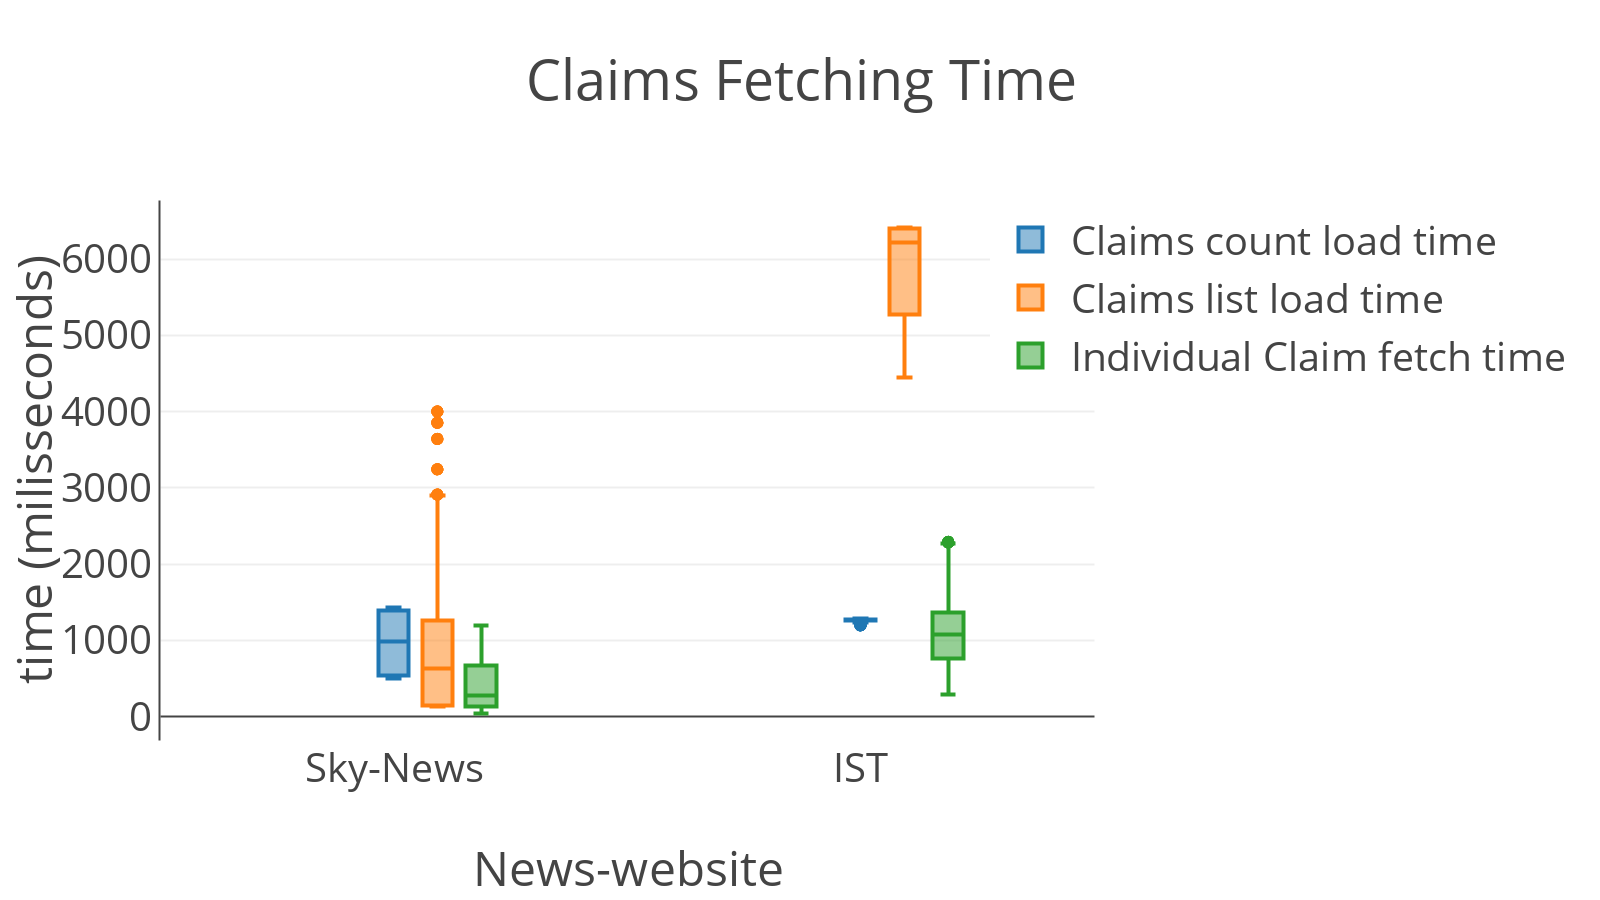
\includegraphics[width=\columnwidth]{figures/chart-fetch.png}
  \vspace{-10pt}
  \caption{Time to retrieve claims on browser.}
%  \vspace{-0.3cm}
  \label{fig:evalclaims}
\end{figure}

\mypara{4. How much time it takes to retrieve the claims of a given article?}
Figure~\ref{fig:evalclaims} shows the time it takes to load a webpage as the number of articles increases. Two curves show the time with and without DClaims.
\fi

\subsection{Performance of the Backend}

We want to evaluate the performance of the backend with respect to the time it takes to retrieve claims.




\mypara{1. What is the claim retrieval time as a function of the number of IPFS nodes in the network?}

Figure \ref{fig:ipfsfetch} shows the time it takes to retrieve individual claims from IPFS. In this experiment we had twenty nodes running DClaims, each node made five claims about random news articles (from a poll of twenty) and then fetched claims from random articles, fetching a new article every ten seconds, for 1400 seconds. \note{fix image x axis label, it should be ten seconds per tick rather than seconds}. Over time the time converges to under ten milliseconds. This happens because of IPFS's cache mechanism, where if a node requests a claim that has requested before, it needs not to ask for it again in the network as a copy is available in their node already. Furthermore, if there are multiple nodes who have the same claim that a given node requests, all those nodes can serve the request.
This chart gives us the following useful information: The longest time that 90\% of the nodes waited for a claim was under one second (outliers were removed ).
Queries are made in parallel, so the time to fetch \textit{n} queries would correspond to the time the slowest query would take.



\subsection{Cost}
Figure \ref{fig:costpublishers} shows the cost of issuing claims in the different available issuance models. The first, individually, corresponds to issuing a claim individually upon its creation. It is the most expensive as it corresponds to the cost of a single issuing transaction (see Table \ref{my-label}), the second one corresponds to the issuance cost if the issuer issued all of his claims once a day (as if he was his own publisher), in this case, the cost is ten times lower, as the transaction cost is divided by the number of claims it carries. Finally, the last modal is using a Publisher, which offers the lowest cost as long as the batch size is higher than the number of claims the person makes in a day.

Figure \ref{fig:timepublishers} shows the confirmation time using the three different issuance mechanisms.
\mypara{Q: How do we know the time it takes with publishers?}
We analyzed three popular news organizations facebook pages and calculated the rate of comments the articles they share receive, which is roughly 4.1 comments per minute. Knowing the batch size in advance, in this case we are using 50, we know the time it takes to fill a batch corresponds to the batch size divided by the rate of claims (which we are assuming is the same as facebook comments).



%!TEX root = ../main.tex

\section{Evaluation}

\note{NS: @João provide a list of the main results we want to add in here.}
\note{TODO: clearly define what are the Qualitative and what are the Quantitative tests}
\note{TODO: add an overview analysis at the end}

\begin{figure}[t]
  \centering 
  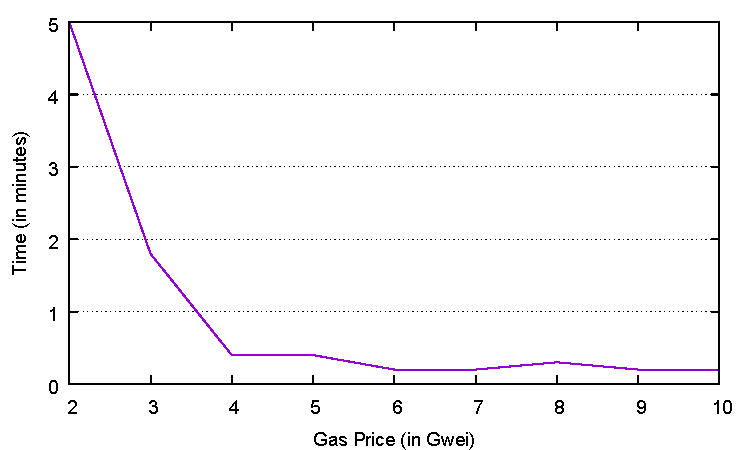
\includegraphics[width=\columnwidth]{final-figures/ethereum-confirmation-time.pdf}
  \vspace{-10pt}
  \caption{Ethereum transaction confirmation time in function of Gas Price.}
%  \vspace{-0.3cm}
  \label{fig:confirmationtime}
\end{figure}

\begin{table}[]
\centering
\begin{tabular}{@{}lll@{}}
\toprule
\textbf{\begin{tabular}[c]{@{}l@{}}Gas price \\ (Gwei)\end{tabular}} & \textbf{\begin{tabular}[c]{@{}l@{}}Contract Creation Cost \\ (in USD)\end{tabular}} & \textbf{\begin{tabular}[c]{@{}l@{}}Claim Issuance Cost\\  (in USD)\end{tabular}} \\ \midrule
\textbf{2}                                                           & 1,72                                                                                & 0,24                                                                             \\
\textbf{4}                                                           & 3,43                                                                                & 0,48                                                                             \\
\textbf{6}                                                           & 5,15                                                                                & 0,72                                                                             \\
\textbf{8}                                                           & 6,86                                                                                & 0,96                                                                             \\
\textbf{10}                                                          & 8,58                                                                                & 1,20                                                                             \\ \bottomrule
\end{tabular}
\caption{DClaims Ethereum Costs}
\label{my-label}
\end{table}


\begin{figure}[t]
  \centering
  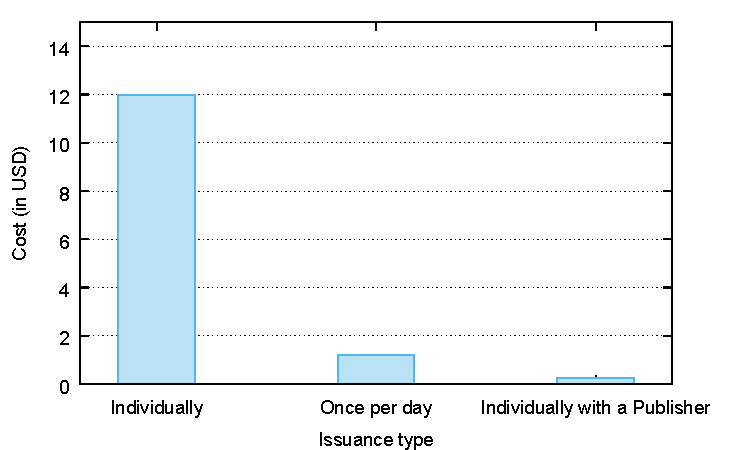
\includegraphics[width=\columnwidth]{final-figures/publisher-issuing-price.pdf}
  \vspace{-10pt}
  \caption{Cost of issuing claims in the different available ways.}
%  \vspace{-0.3cm}
  \label{fig:costpublishers}
\end{figure}

\begin{figure}[t]
  \centering
  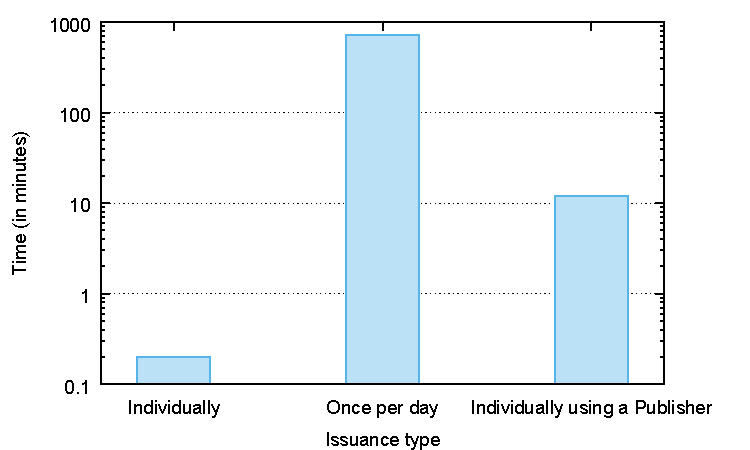
\includegraphics[width=\columnwidth]{final-figures/publisher-issuing-time.pdf}
  \vspace{-10pt}
  \caption{Time for claims to be confirmed on the Ethereum blockchain}
%  \vspace{-0.3cm}
  \label{fig:timepublishers}
\end{figure}

\begin{figure}[t]
  \centering
  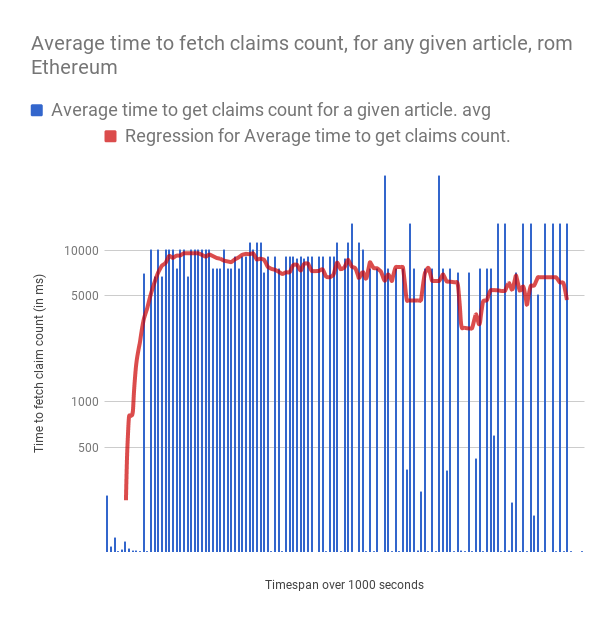
\includegraphics[width=\columnwidth]{mock-figures/ethereumfetch.png}
  \vspace{-10pt}
  \caption{Time to load a webpage as function of the number of articles. \note{NS: @João dont forget to add two curves: one with the other without DClaims.}}
%  \vspace{-0.3cm}
  \label{fig:ethereumfetch}
\end{figure}

\begin{figure}[t]
  \centering
  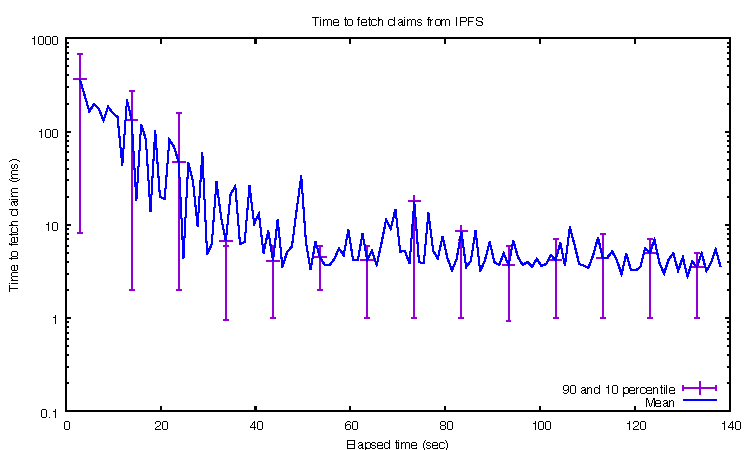
\includegraphics[width=\columnwidth]{mock-figures/ipfsfetch.pdf}
  \vspace{-10pt}
  \caption{Time to fetch individual claims from IPFS}
%  \vspace{-0.3cm}
  \label{fig:ipfsfetch}
\end{figure}

\subsection{Performance of Web Application}


In this section, we evaluate the impact of DClaims in terms of the user experience of the website. \note{NS: @João extend the same experiments for 5 sites, try to pick different sites.}

\begin{figure}[t]
  \centering
  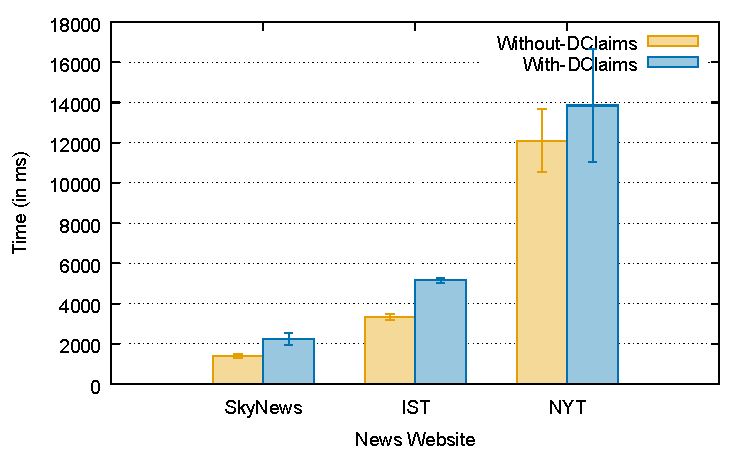
\includegraphics[width=\columnwidth]{final-figures/website-3-comparison.pdf}
  \vspace{-10pt}
  \caption{Loading time comparison of popular news websites with and without DClaims running.}
%  \vspace{-0.3cm}
  \label{fig:evalwebpage}
\end{figure}

\mypara{1. What's the overhead of loading a web page with DClaims?} Figure~\ref{fig:evalwebpage} shows the time it takes to fetch claims from three news websites, Instituto Superior Técnico, SkyNews and New York Times. We can see that the overhead introduced by DClaims is very low.

Figure \ref{fig:evalnarticles} is a benchmark test were we used a striped down version of a website as a basis and created several versions of that website, each with ten more news articles than the previous one. As the figure shows the overhead introduced by DClaims is proportional to the number of articles per page.

By comparing Figures \ref{fig:evalwebpage} and \ref{fig:evalnarticles} one might wonder why in the first, the overhead introduced by DClaims appears to be smaller than in the second. That happens because the website we used for the benchmark has been stripped down of any Javascript code, which slows down the loading time. The same does not happen in regular websites such as SkyNews and the New York Times. 

\note{JS: The conclusion here is that while when compared to super simplified websites, the overhead introduced by DClaims is significant, in the real world it is hardly noticed because regular websites are loaded with JS code that slows down the loading time}

\begin{figure}[t]
  \centering
  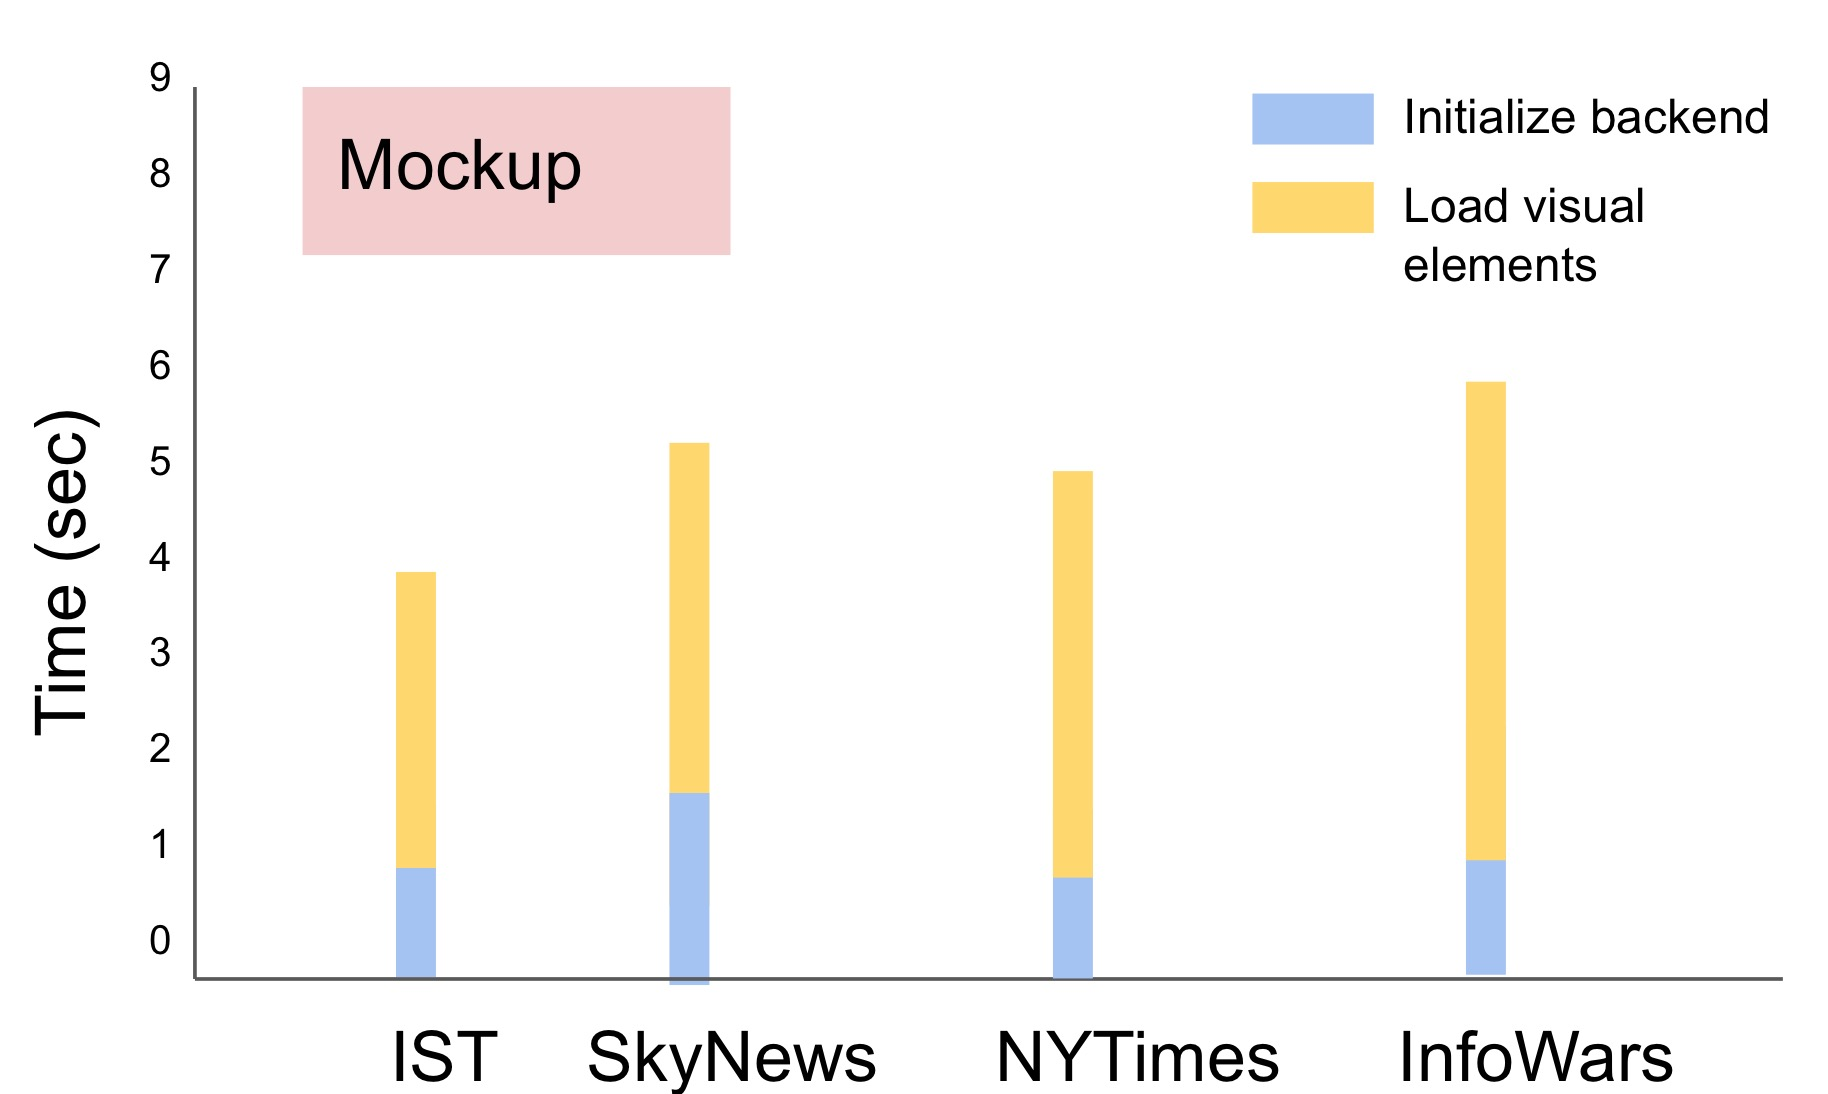
\includegraphics[width=\columnwidth]{mock-figures/timessubcomponents.jpg}
  \vspace{-10pt}
  \caption{Time of drawing the elements and initializing the backend.}
%  \vspace{-0.3cm}
  \label{fig:evalpartial}
\end{figure}

\mypara{2. What is the source of the overheads introduced by DClaims?} Figure~\ref{fig:evalpartial} shows the contributions of two main parts: element drawing and interaction with the backend. \note{NS: @João please change the graph to a compound graph.}
 \note{JS: Didn't have the time to do this one yet}


\begin{figure}[t]
  \centering
  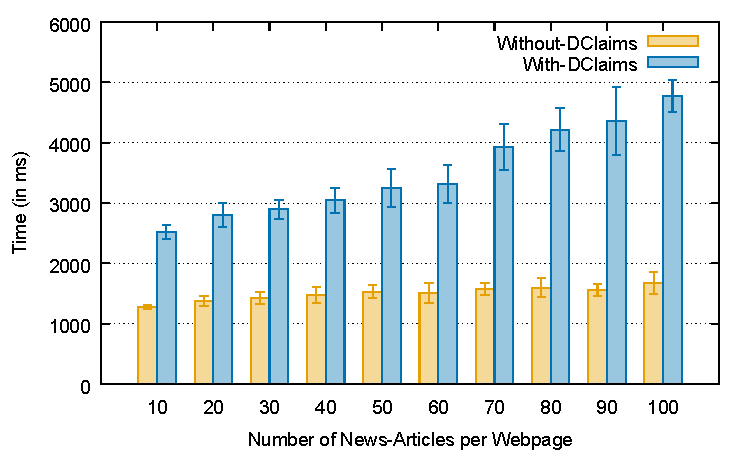
\includegraphics[width=\columnwidth]{final-figures/website-benchmark.pdf}
  \vspace{-10pt}
  \caption{Time to load a webpage as function of the number of articles.}
%  \vspace{-0.3cm}
  \label{fig:evalnarticles}
\end{figure}


\mypara{3. What is the website loading time based on the number of articles in the page?} Figure~\ref{fig:evalnarticles} shows the graph.

\note{JS: I believe this question is answered in the first question " What's the overhead of loading a web page with DClaims?"}

\if0
\begin{figure}[t]
  \centering
  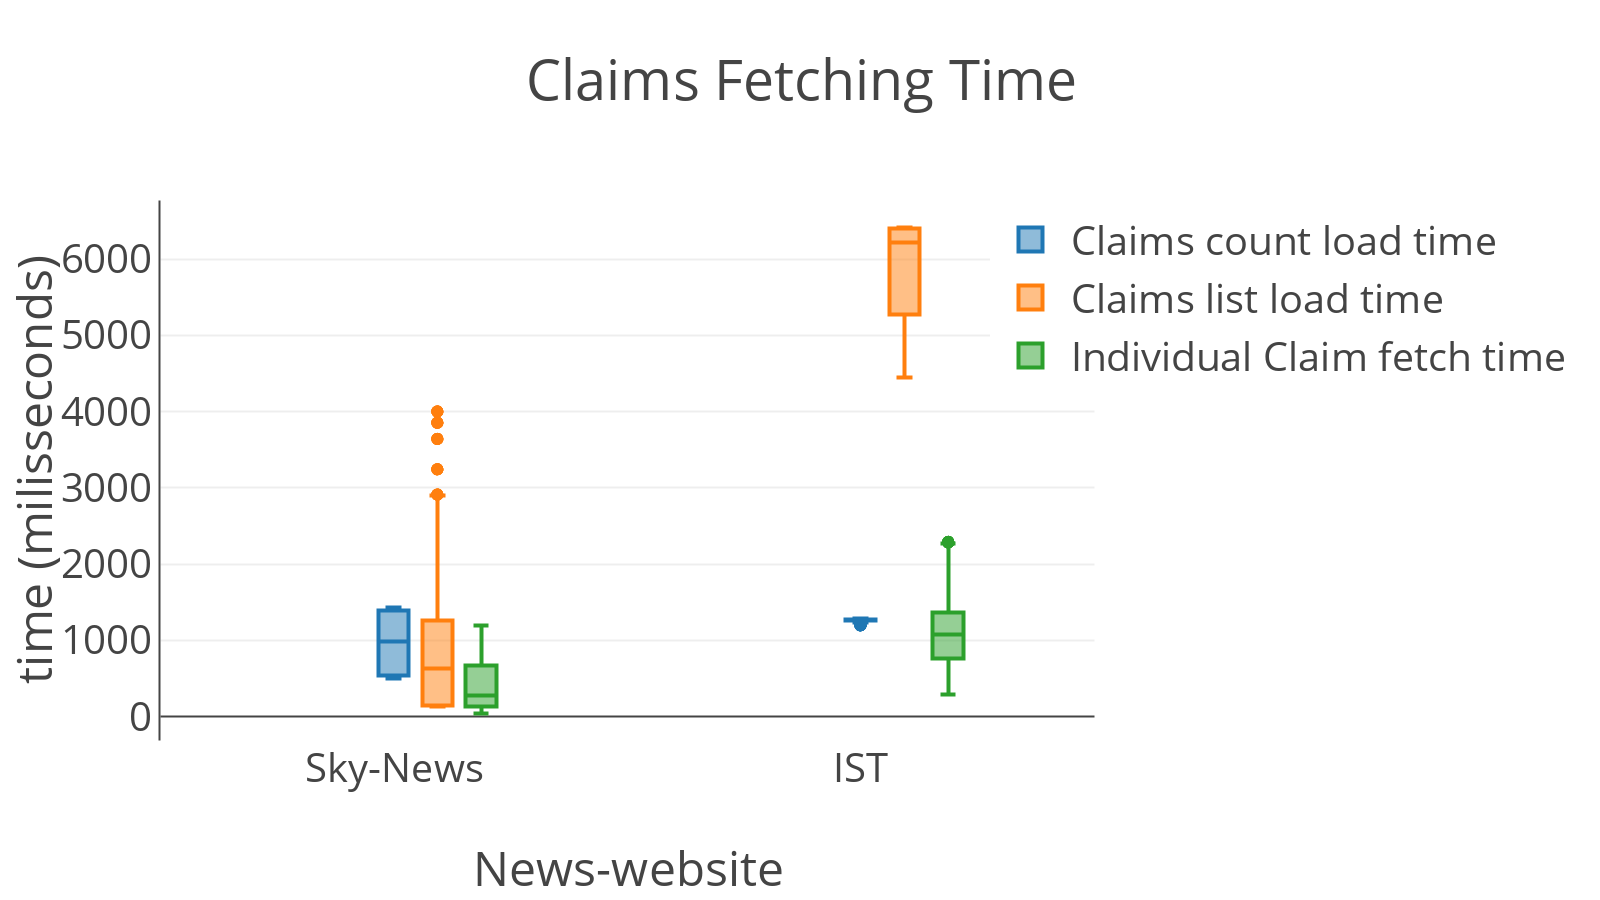
\includegraphics[width=\columnwidth]{figures/chart-fetch.png}
  \vspace{-10pt}
  \caption{Time to retrieve claims on browser.}
%  \vspace{-0.3cm}
  \label{fig:evalclaims}
\end{figure}

\mypara{4. How much time it takes to retrieve the claims of a given article?}
Figure~\ref{fig:evalclaims} shows the time it takes to load a webpage as the number of articles increases. Two curves show the time with and without DClaims.
\fi

\subsection{Performance of the Backend}

We want to evaluate the performance of the backend with respect to the time it takes to retrieve claims.




\mypara{1. What is the claim retrieval time as a function of the number of IPFS nodes in the network?}

Figure \ref{fig:ipfsfetch} shows the time it takes to retrieve individual claims from IPFS. In this experiment we had twenty nodes running DClaims, each node made five claims about random news articles (from a poll of twenty) and then fetched claims from random articles, fetching a new article every ten seconds, for 1400 seconds. \note{fix image x axis label, it should be ten seconds per tick rather than seconds}. Over time the time converges to under ten milliseconds. This happens because of IPFS's cache mechanism, where if a node requests a claim that has requested before, it needs not to ask for it again in the network as a copy is available in their node already. Furthermore, if there are multiple nodes who have the same claim that a given node requests, all those nodes can serve the request.
This chart gives us the following useful information: The longest time that 90\% of the nodes waited for a claim was under one second (outliers were removed ).
Queries are made in parallel, so the time to fetch \textit{n} queries would correspond to the time the slowest query would take.



\subsection{Cost}
Figure \ref{fig:costpublishers} shows the cost of issuing claims in the different available issuance models. The first, individually, corresponds to issuing a claim individually upon its creation. It is the most expensive as it corresponds to the cost of a single issuing transaction (see Table \ref{my-label}), the second one corresponds to the issuance cost if the issuer issued all of his claims once a day (as if he was his own publisher), in this case, the cost is ten times lower, as the transaction cost is divided by the number of claims it carries. Finally, the last modal is using a Publisher, which offers the lowest cost as long as the batch size is higher than the number of claims the person makes in a day.

Figure \ref{fig:timepublishers} shows the confirmation time using the three different issuance mechanisms.
\mypara{Q: How do we know the time it takes with publishers?}
We analyzed three popular news organizations facebook pages and calculated the rate of comments the articles they share receive, which is roughly 4.1 comments per minute. Knowing the batch size in advance, in this case we are using 50, we know the time it takes to fill a batch corresponds to the batch size divided by the rate of claims (which we are assuming is the same as facebook comments).


%!TEX root = ../main.tex

\section{Conclusions}

Write me. \note{NS: save it for last}


{\footnotesize \bibliographystyle{acm}
\bibliography{main}}

\end{document}
